%% COV-DVG: A Learned Value Gate for Cost-Aware Multi-Agent LLM Debate
%% IEEE conference paper (IEEEtran). Compile: pdflatex main.tex (x2).
\documentclass[conference]{IEEEtran}
\IEEEoverridecommandlockouts

\usepackage{cite}
\usepackage{amsmath,amssymb,amsfonts}
\usepackage{algorithmic}
\usepackage{graphicx}
\usepackage{booktabs}
\usepackage{array}
\usepackage{stfloats}   % better placement of double-column figure* floats
\usepackage{xcolor}
\usepackage{url}
\usepackage[hidelinks]{hyperref}

\begin{document}

\title{When Is Debate Worth It? A Learned Value Gate\\ for Cost-Aware Multi-Agent LLM Debate}

\author{\IEEEauthorblockN{Simon Dagbanja}
\IEEEauthorblockA{\textit{Independent Researcher}\\
Email: simondagbanja258@gmail.com}}

\maketitle

\begin{abstract}
Multi-agent debate can raise the accuracy of large language models (LLMs), but it
multiplies inference cost and its benefit is highly uneven across tasks; recent work
even reports that debate can \emph{degrade} accuracy. We ask a practical question:
\emph{given a problem, is debating worth its token cost?} We present COV-DVG, a
learned \emph{value gate} that predicts, from pre-debate observable features alone
(no ground-truth leakage), whether a critic--adjudicator debate will correct,
preserve, or subvert the majority answer, together with its token cost, and debates
only when the expected accuracy gain justifies the spend. Using Qwen3-14B (4-bit
AWQ) served with vLLM across GSM8K, MMLU-Pro, MATH, and GPQA, we find that debate's
value is concentrated on \emph{procedural} reasoning (MATH: $+0.07$ accuracy over
majority voting, $p<10^{-4}$) and is essentially absent on \emph{knowledge-recall}
tasks (GPQA, MMLU-Pro), where the best-possible debate policy exceeds the base solver
by only $2$--$3$ points. The gate exploits this structure: it debates MATH almost
always and correctly abstains on the knowledge-bound benchmarks, matching
always-debate accuracy while saving $44$--$63\%$ of debate tokens. An optional
sandboxed code-execution verifier extends debate's reach on the computational subset
of MATH (oracle $0.867\!\rightarrow\!0.880$). Finally, we document and quantify a
subtle evaluation hazard---generation truncation---that inflates the apparent value
of debate for spurious reasons, and show that removing it changes the qualitative
conclusions.
\end{abstract}

\begin{IEEEkeywords}
large language models, multi-agent debate, adaptive inference, inference cost,
tool use, self-consistency
\end{IEEEkeywords}

\section{Introduction}
Prompting large language models (LLMs) to reason step by step~\cite{wei2022cot} and
aggregating multiple sampled reasoning paths~\cite{wang2023selfcons,li2024moreagents}
are now standard ways to raise accuracy on hard tasks. \emph{Multi-agent debate}
extends this idea: several LLM ``solvers'' propose answers that are then reconciled
through structured critique and adjudication~\cite{du2024debate,liang2024mad,
wang2024moa}. Reported gains, however, come at a steep and often \emph{unnecessary}
cost---every debated problem incurs several extra generations---and the benefit is
far from universal. Indeed, recent analyses show debate can \emph{reduce} accuracy,
as models favor social agreement over challenging flawed
reasoning~\cite{wynn2025failure}. Whether debate helps therefore depends on the
problem, and spending debate compute uniformly is wasteful.

We study a cost-aware alternative. A \emph{value gate} inspects only the information
available \emph{before} any debate output exists---the distribution of independent
answers, their agreement and confidence, and cheap textual features---and predicts
the \emph{outcome} of debating (correction, no change, or subversion) as well as its
token cost. The gate debates a problem only when the expected accuracy gain outweighs
a small token penalty. Because the gate never sees ground truth or any post-debate
signal, its decisions are deployable at inference time. This connects debate to the
literature on adaptive and cascaded inference~\cite{chen2023frugalgpt}, but routes
the \emph{debate decision} rather than the model.

Our contributions are:
\begin{itemize}
\item \textbf{COV-DVG}, a learned dual-head value gate (outcome $+$ cost) trained on
observed debate outcomes, with a per-benchmark operating point selected on held-out
validation data (Section~\ref{sec:method}).
\item An empirical characterization of \emph{when} debate helps: with a strong 14B
solver, debate value is large on procedural reasoning (MATH) and near-zero on
knowledge recall (GPQA, MMLU-Pro). The gate captures this, matching always-debate
accuracy at $44$--$63\%$ lower token cost where debate is unhelpful, and
significantly beating majority voting where it is (Section~\ref{sec:results}).
\item An optional \textbf{sandboxed code-execution verifier} that raises the debate
ceiling on the computational subset of MATH, in the spirit of program-aided
reasoning~\cite{gao2023pal,chen2023pot}.
\item A cautionary result: an easily-overlooked \textbf{generation-truncation}
artifact can make debate appear beneficial for the wrong reasons; we quantify it and
show it must be controlled for.
\end{itemize}

\section{Related Work}
\textbf{Ensembling and debate.} Self-consistency marginalizes over sampled reasoning
paths~\cite{wang2023selfcons}, and simple sampling-and-voting scales with the number
of agents~\cite{li2024moreagents}. Multi-agent debate adds structured interaction:
agents critique and revise across rounds~\cite{du2024debate,liang2024mad}, and
layered mixtures of agents further improve quality~\cite{wang2024moa}. Self-refinement
achieves related gains with a single model acting as generator, critic, and
reviser~\cite{madaan2023selfrefine}. A growing body of work tempers these claims:
debate can be harmful when weaker agents are present or when models conform to
incorrect peers~\cite{wynn2025failure}. Our work is orthogonal to the debate protocol
itself---we learn \emph{when} to invoke one, and quantify where its value actually
lies.

\textbf{Adaptive and cost-aware inference.} LLM cascades route easy queries to cheap
models and hard ones to expensive models to cut cost~\cite{chen2023frugalgpt}.
COV-DVG applies the same economic logic to the debate decision, using outcome
prediction from pre-debate features rather than a difficulty proxy.

\textbf{Tool-augmented reasoning.} Program-aided and program-of-thought methods
offload computation to an interpreter, disentangling reasoning from
arithmetic~\cite{gao2023pal,chen2023pot}. We use a sandboxed verifier as
\emph{evidence} for adjudication rather than as the primary solver, which lets the
adjudicator ignore incorrect or crashing programs.

\section{Method}
\label{sec:method}
COV-DVG turns each problem into an \emph{episode} and learns a gate over episodes.
The pipeline preserves two invariants: (i) solvers, critic, and adjudicator never see
ground truth; (ii) the gate conditions only on pre-debate observable features.

\subsection{Independent solver panel}
For a problem $x$ we draw $K{=}5$ role-conditioned solvers (independent solver,
skeptical verifier, formal analyst, alternative-method solver, examiner). Each
produces a solution ending in a mechanically gradable \texttt{FINAL} line and a
self-reported \texttt{CONFIDENCE}. Answers are grouped by task-aware equivalence into
a \emph{semantic majority} $\hat{y}_\text{maj}$, the base answer---a debate-free
baseline equivalent to self-consistency over heterogeneous roles~\cite{wang2023selfcons}.

\subsection{Critic--adjudicator debate}
An adversarial \emph{critic} inspects the candidate solutions for concrete errors
without access to an answer key. A final \emph{adjudicator} independently
re-verifies, using the panel and the critique only when they are correct, and emits
the debate answer $\hat{y}_\text{deb}$. Neither stage is told the majority is
authoritative, which limits the conformity failure mode of~\cite{wynn2025failure}.

\subsection{Pre-debate features and outcome labels}
From the panel alone we extract a $24$-dimensional feature vector $\phi(x)$:
agreement statistics (top-vote share, vote margin, answer entropy, diversity,
consensus indicator), confidence statistics (mean/std, majority vs.\ minority
confidence and their gap, confidence--vote correlation), response-length and
pairwise reasoning-similarity features, a \emph{parse-failure rate}, and benchmark
indicators. Grading (which uses ground truth) produces the observed \emph{outcome
label}
\[
\delta = \mathbb{1}[\hat{y}_\text{deb}=y] - \mathbb{1}[\hat{y}_\text{maj}=y]\in\{-1,0,+1\},
\]
i.e.\ \emph{subversion}, \emph{no-change}, or \emph{correction}, and the debate token
cost $c(x)$. Labels are used only to \emph{train} the gate, never at decision time.

\subsection{The neural value gate}
The gate is a dual-head multilayer perceptron (hidden sizes $[128,64]$, LayerNorm,
dropout $0.2$) on standardized features. An outcome head predicts a distribution over
$\{-1,0,+1\}$; a cost head regresses $\log(1+c)$. We minimize a class-weighted
cross-entropy (to counter the rarity of corrections/subversions) plus a smooth-$L_1$
cost loss, optimized with AdamW for $120$ epochs under a plateau learning-rate
scheduler; the best-validation checkpoint is restored. At decision time the gate
forms a utility
\[
u(x) = P(\text{correction}) - P(\text{subversion}) - \lambda\,\hat{c}(x)/1000,
\]
and debates iff $u(x) > \tau$. The threshold $\tau$ is tuned on validation to
maximize a token-penalized accuracy, \emph{per benchmark} with a global fallback, so
that benchmarks on which debate helps broadly may debate freely while others abstain.

\subsection{Optional code-execution verifier}
For computational tasks (MATH, GSM8K), an optional stage inserts a ``programmer''
between critic and adjudicator: it writes a short, self-contained Python/SymPy
program that recomputes the answer, in the spirit of PAL and Program-of-Thoughts
prompting~\cite{gao2023pal,chen2023pot}. The program runs in a sandbox (isolated
subprocess, wall-clock timeout, Linux CPU/address-space limits, math libraries only)
and its printed result is handed to the adjudicator as \emph{evidence to verify}---
never as ground truth, since the code may be wrong or crash. Its token cost is folded
into the debate cost for fair accounting.

\section{Experimental Setup}
\label{sec:setup}
\textbf{Benchmarks.} GSM8K (grade-school arithmetic)~\cite{cobbe2021gsm8k}, MMLU-Pro
(ten-option knowledge MCQ)~\cite{wang2024mmlupro}, MATH (competition
mathematics)~\cite{hendrycks2021math}, and GPQA (graduate-level science
MCQ)~\cite{rein2023gpqa}; for GPQA we use the larger \emph{main} split for
statistical power. Test sizes are $200/200/300/200$. Official train/validation pools
are used to fit and tune the gate; train/validation and test pools are permanently
disjoint.

\textbf{Model and serving.} Qwen3-14B~\cite{qwen2025qwen3}, 4-bit
AWQ-quantized~\cite{lin2024awq}, in non-thinking mode, served with vLLM using
PagedAttention~\cite{kwon2023vllm} on a single 24\,GB GPU. Per-task generation budgets
(GSM8K $320$, MATH $768$, MCQ $1024$ tokens; critic $512$, judge $768$) prevent
truncation (Section~\ref{sec:trunc}). Decoding uses temperature $0.7$ for solvers and
lower temperatures for critic/judge.

\textbf{Metrics and baselines.} Beyond majority voting~\cite{wang2023selfcons} and
always-debate~\cite{du2024debate}, we report \emph{matched-rate} heuristics that
debate the same number of items as the gate but choose them by answer entropy
(uncertainty), majority confidence (low-confidence), or at random; and an
\emph{oracle} that debates exactly the items debate would help. We report accuracy,
token cost, paired bootstrap $95\%$ confidence intervals ($2000$ resamples), and exact
McNemar $p$-values.

\section{Results}
\label{sec:results}

\subsection{A truncation artifact that must be controlled}
\label{sec:trunc}
Before the main results we flag a hazard. With an aggressive generation cap, solvers
on the hardest benchmarks exhausted their token budget mid-reasoning and never emitted
a parseable \texttt{FINAL}/\texttt{CONFIDENCE} line. Table~\ref{tab:trunc} shows the
effect on GPQA: two-thirds of agent answers were unparseable, all confidences collapsed
to the $0.5$ default, and the base accuracy fell \emph{below} the random floor
($0.25$). In this regime debate ``helps'' largely by cleaning up formatting failures
rather than by reasoning---an artifact that flatters debate and can masquerade as the
gains reported in the literature. Raising per-task budgets removes it (empty-answer rate
$0.65\!\rightarrow\!0.00$; generated length no longer at the cap). All subsequent
results use the un-truncated configuration.

\begin{table}[!t]
\caption{Generation truncation is an evaluation hazard (GPQA).}
\label{tab:trunc}
\centering
\begin{tabular}{lcc}
\toprule
 & Truncated (256 tok) & Fixed (per-task) \\
\midrule
Empty agent answers      & $0.65$ & $0.00$ \\
Agent confidences alive  & no ($\equiv 0.5$) & yes \\
Base (majority) accuracy & $0.10$ & $0.41$ \\
\bottomrule
\end{tabular}
\end{table}

\subsection{Main results}
Table~\ref{tab:main} reports the full comparison for COV-DVG (14B\,$+$\,tools).
COV-DVG never loses to majority voting and, crucially, \emph{matches} always-debate
accuracy within noise on every benchmark while spending far fewer tokens on three of
four. On MATH it beats majority by $+0.07$ ($p=4.9\times10^{-5}$, CI
$[0.04,0.10]$). On GSM8K and MMLU-Pro it abstains entirely, saving $63\%$ and $57\%$
of the tokens always-debate would spend, at no significant accuracy cost.

\begin{table*}[!t]
\caption{Primary test results with COV-DVG (Qwen3-14B AWQ $+$ code-execution verifier).
Accuracies are fractions; ``Save'' is token savings vs.\ always-debate; ``$\Delta$maj''
is the paired difference vs.\ majority with a $95\%$ bootstrap CI; $p_\text{maj}$ is the
exact McNemar $p$-value vs.\ majority. Matched-rate baselines (Unc., Rand.) debate the
same number of items as COV-DVG.}
\label{tab:main}
\centering
\begin{tabular}{lccccccccccc}
\toprule
Benchmark & $n$ & Majority & Always & \textbf{COV-DVG} & Unc.\ & Rand.\ & Oracle & Rate & Save & $\Delta$maj (CI) & $p_\text{maj}$ \\
\midrule
GSM8K    & 200 & 0.935 & 0.950 & \textbf{0.935} & 0.935 & 0.935 & 0.950 & 0.00 & $63.2\%$ & $0.00\ [0.00,0.00]$ & $1.0$ \\
MMLU-Pro & 200 & 0.690 & 0.695 & \textbf{0.690} & 0.690 & 0.690 & 0.715 & 0.00 & $57.2\%$ & $0.00\ [0.00,0.00]$ & $1.0$ \\
MATH     & 300 & 0.800 & 0.870 & \textbf{0.870} & 0.870 & 0.870 & 0.880 & 0.99 & $0.5\%$  & $0.07\ [0.04,0.10]$ & $4.9\!\times\!10^{-5}$ \\
GPQA     & 200 & 0.460 & 0.485 & \textbf{0.460} & 0.475 & 0.465 & 0.490 & 0.22 & $44.0\%$ & $0.00\ [0.00,0.00]$ & $1.0$ \\
\bottomrule
\end{tabular}
\end{table*}

\subsection{When does debate help? Procedural vs.\ knowledge tasks}
The key explanatory quantity is the \emph{debate headroom}, oracle minus base
accuracy---the most any gate could gain. Table~\ref{tab:headroom} shows it is large
only on MATH. On GSM8K, MMLU-Pro, and GPQA the oracle exceeds the base solver by just
$1$--$3$ points: a strong model's errors on these benchmarks are \emph{knowledge
gaps}, and self-debate cannot supply knowledge the model lacks. On MATH the errors are
\emph{procedural} (arithmetic/algebra slips) that re-derivation fixes. This is the
central finding: \emph{debate is valuable for procedural reasoning and largely inert
for knowledge recall}, and a learned gate should---and does---route accordingly.
Fig.~\ref{fig:policy} makes the same point geometrically: MATH accuracy climbs steeply
with debate rate (the gate's operating point sits at the top), while the knowledge
benchmarks are nearly flat, so the gate parks them at rate $0$.

\begin{table}[!t]
\caption{Debate headroom (oracle $-$ base) explains the gate's policy.}
\label{tab:headroom}
\centering
\begin{tabular}{lccc}
\toprule
Benchmark & Base & Oracle & Headroom \\
\midrule
MATH     & 0.800 & 0.880 & $\mathbf{+0.080}$ \\
GPQA     & 0.460 & 0.490 & $+0.030$ \\
MMLU-Pro & 0.690 & 0.715 & $+0.025$ \\
GSM8K    & 0.935 & 0.950 & $+0.015$ \\
\bottomrule
\end{tabular}
\end{table}

\subsection{The gate is genuinely learning}
Fig.~\ref{fig:train} shows training dynamics. The dual losses converge by
$\sim\!20$ epochs; the plateau scheduler then reduces the learning rate three times.
Validation gate accuracy sits well above majority and just under always-debate and the
oracle throughout, and the value-add (gate $-$ majority) is stable and positive. Train
accuracy drifts upward (mild over-fitting on a small, class-imbalanced episode set),
which is why we restore the best-validation checkpoint (epoch $20$).

\subsection{Scaling and the value of fixing the sensor}
Table~\ref{tab:scaling} traces base (majority) accuracy across solver models. The
largest gains come from (i) removing the truncation artifact and (ii) scaling the
solver from $4$B to $14$B, not from the debate machinery. This reinforces the main
finding: with a capable base solver, the accuracy ceiling on knowledge benchmarks is
set by model knowledge, and debate's role narrows to procedural tasks and to cost
economization.

\begin{table}[!t]
\caption{Base (majority) accuracy by solver model~\cite{qwen2025qwen3}. GPQA uses the
\emph{diamond} split for 4B/8B and the larger \emph{main} split for 14B (marked
$^{\dagger}$), so its column is not strictly comparable across rows.}
\label{tab:scaling}
\centering
\begin{tabular}{lcccc}
\toprule
Solver & GSM8K & MMLU-Pro & MATH & GPQA \\
\midrule
Qwen3-4B (truncated)  & 0.75 & 0.19 & 0.26 & 0.10 \\
Qwen3-8B              & 0.93 & 0.63 & 0.73 & 0.41 \\
Qwen3-14B             & 0.94 & 0.69 & 0.80 & $0.46^{\dagger}$ \\
\bottomrule
\end{tabular}
\end{table}

\subsection{Code-execution verifier ablation}
Table~\ref{tab:tools} isolates the verifier. On MATH it lifts always-debate
$0.860\!\rightarrow\!0.870$ and, more tellingly, the \emph{oracle}
$0.867\!\rightarrow\!0.880$: the tool solves items neither the panel nor plain debate
could, breaking the self-debate ceiling. The gain is real but modest. Diagnostics
explain why: the generated program executes cleanly $88\%$ of the time but is correct
only $69\%$---below the panel's $80\%$---because much of MATH (proofs, symbolic
expressions, geometry) is not cleanly computable, unlike the numeric benchmarks PAL and
PoT target~\cite{gao2023pal,chen2023pot}. The verifier's value is thus as a
\emph{selectively trusted cross-check} (the adjudicator adopts its answer only $43\%$
of the time), recovering $35\%$ of otherwise-wrong items.

\begin{table}[!t]
\caption{Effect of the code-execution verifier (14B).}
\label{tab:tools}
\centering
\begin{tabular}{llcc}
\toprule
Benchmark & Metric & 14B & 14B\,$+$\,tools \\
\midrule
MATH  & always-debate & 0.860 & \textbf{0.870} \\
MATH  & oracle        & 0.867 & \textbf{0.880} \\
MATH  & COV-DVG       & 0.860 & \textbf{0.870} \\
GSM8K & always-debate & 0.945 & \textbf{0.950} \\
\bottomrule
\end{tabular}
\end{table}

\section{Discussion and Limitations}
\textbf{Interpretation.} The practical takeaway is a routing rule: spend debate compute
where errors are procedural and verifiable, and abstain where they are knowledge-bound.
COV-DVG learns this rule from cheap pre-debate signals and, at its selected operating
points, delivers always-debate accuracy at a fraction of the cost on three of four
benchmarks and a significant accuracy gain on the fourth. This complements reports that
debate is not universally beneficial~\cite{wynn2025failure} by giving a deployable
criterion for when to use it.

\textbf{Limitations.} (i) The gate trains on a few hundred episodes with rare
correction/subversion labels; outcome macro-$F_1$ is modest and the learned policy is
effectively a well-calibrated per-benchmark threshold rather than a fine-grained
per-item selector. (ii) GPQA remains knowledge-bound: no debate or tool strategy we
tried moves its $\sim\!0.49$ oracle; retrieval augmentation or a larger solver is the
only lever. (iii) The GPQA split differs across scaling rows. (iv) Results use one
model family on a single GPU; absolute numbers will shift with model and decoding.

\textbf{Future work.} Retrieval-augmented debate to raise the knowledge ceiling on
GPQA/MMLU-Pro; richer per-item gating with more episodes; and extending the verifier
toward symbolic proof checking.

\section{Conclusion}
We presented COV-DVG, a learned value gate that decides when multi-agent debate is
worth its cost using only pre-debate features. Across four benchmarks with a strong 14B
solver, we showed that debate's value is concentrated on procedural reasoning and
near-zero on knowledge recall, and that the gate exploits this to match always-debate
accuracy while saving $44$--$63\%$ of debate tokens where debate is unhelpful and to
significantly beat majority voting where it is. A sandboxed code-execution verifier
extends debate's reach on computational problems. We also cautioned that a simple
generation-truncation artifact can inflate the apparent value of debate and must be
controlled for.

% ---- Wide (double-column) figures. Placed here and flushed before the
% ---- bibliography so no float ever follows the reference list.
\begin{figure*}[!t]
\centering
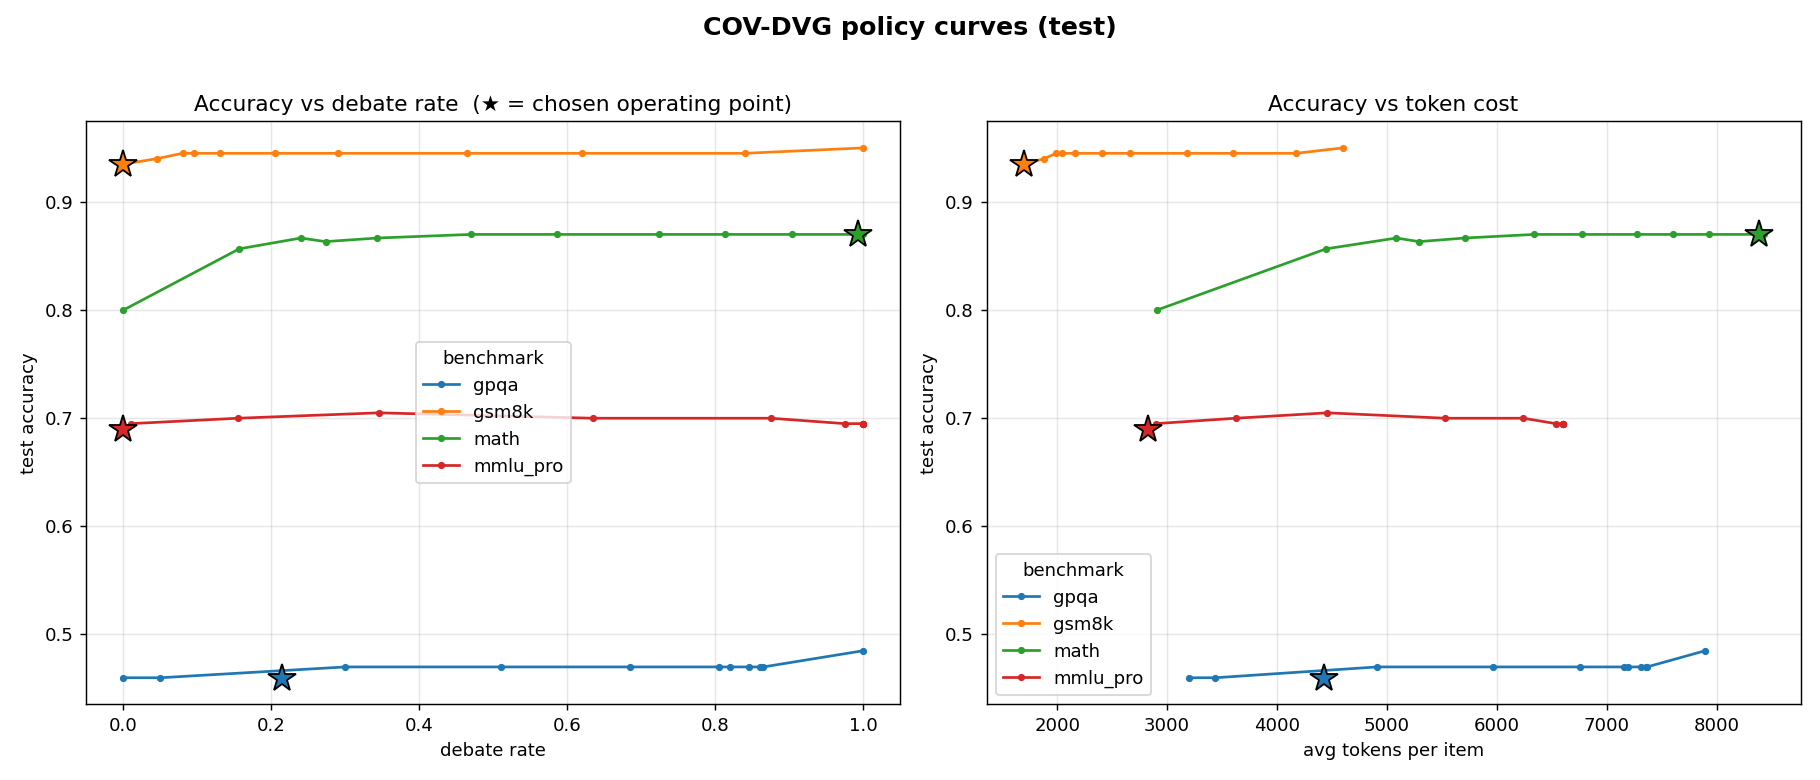
\includegraphics[width=\textwidth]{figs/policy_curves.png}
\caption{Test accuracy vs.\ debate rate (left) and vs.\ token cost (right), with
thresholds swept from validation quantiles. The star marks the gate's chosen operating
point. MATH (green) rises steeply---debate has real headroom and the gate debates it
fully; the knowledge benchmarks are nearly flat, so the gate abstains and saves tokens.
GSM8K (orange) saturates immediately.}
\label{fig:policy}
\end{figure*}

\begin{figure*}[!t]
\centering
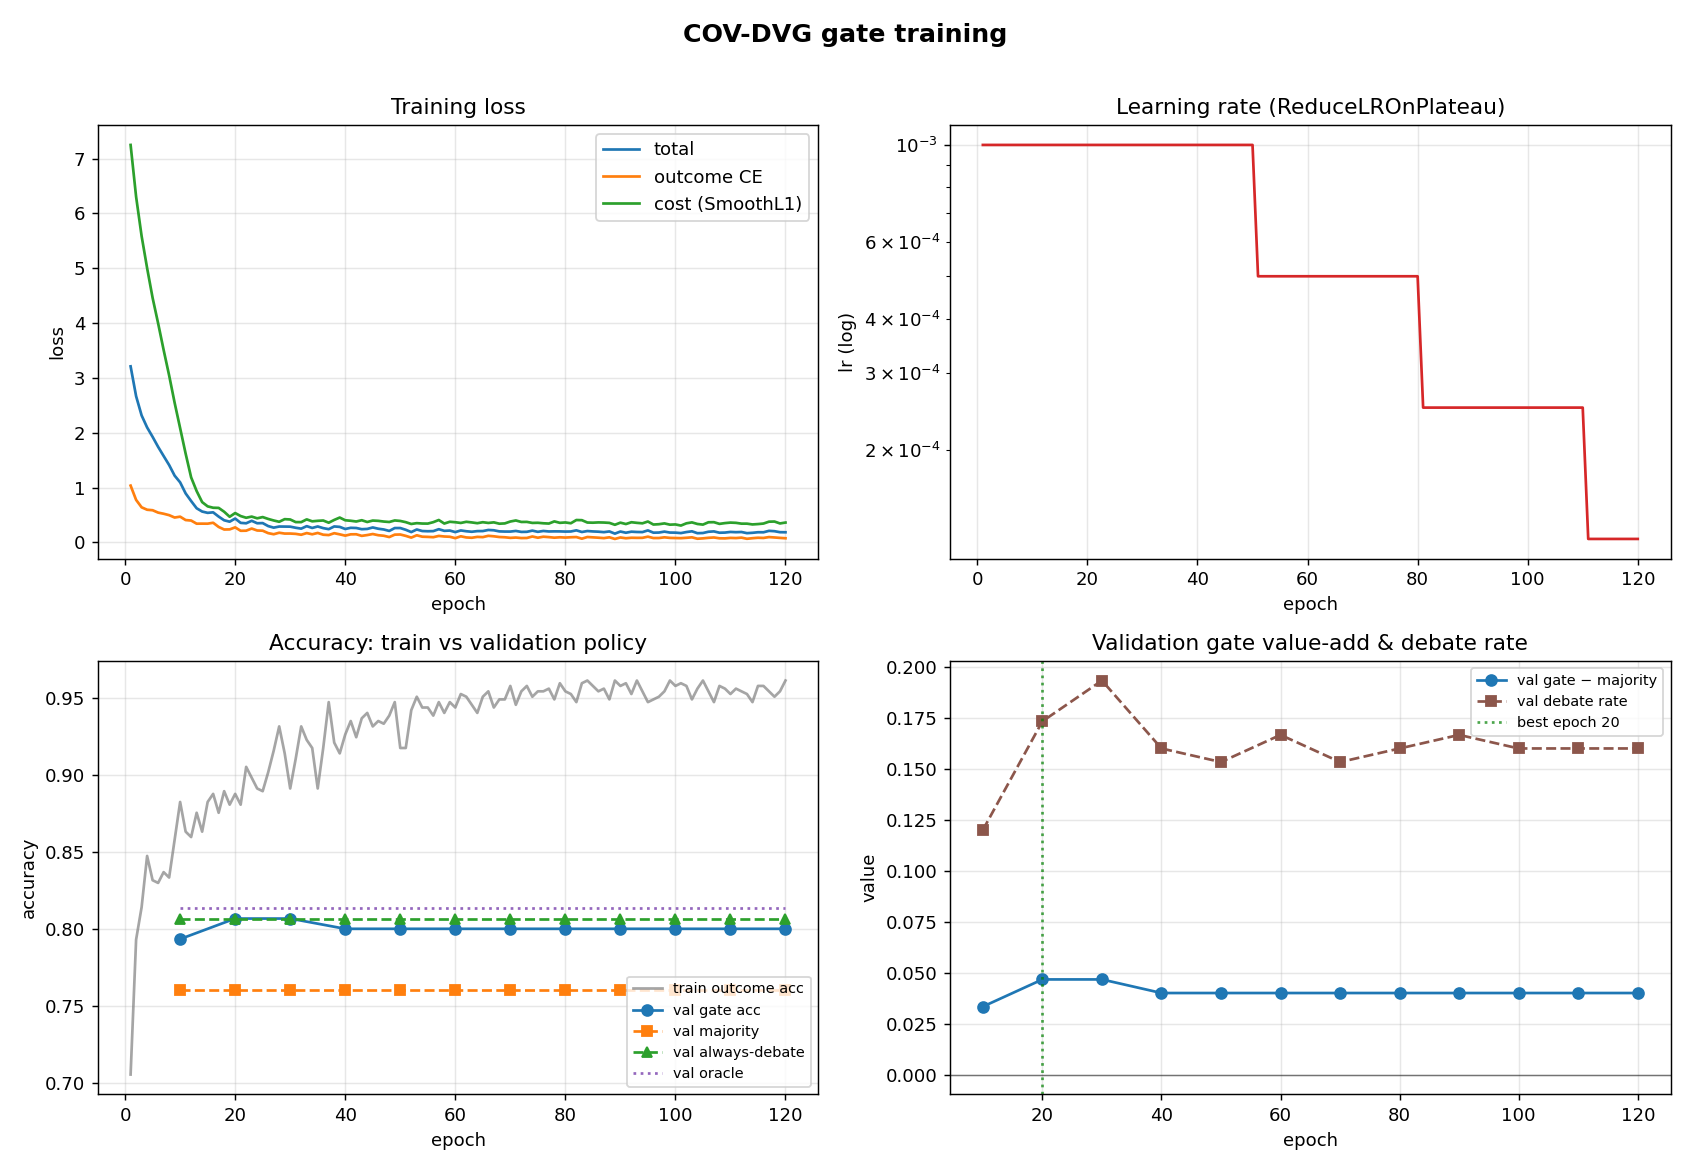
\includegraphics[width=\textwidth]{figs/training_curves.png}
\caption{Gate training. Top: loss components and the plateau learning-rate schedule.
Bottom: validation gate accuracy vs.\ majority/always-debate/oracle references, and the
validation value-add with the selected best epoch.}
\label{fig:train}
\end{figure*}

\clearpage  % flush all pending floats so none appears after the references

\begin{thebibliography}{18}
\bibitem{wei2022cot} J.~Wei \emph{et al.}, ``Chain-of-thought prompting elicits
reasoning in large language models,'' in \emph{Adv. Neural Inf. Process. Syst.
(NeurIPS)}, 2022. arXiv:2201.11903.
\bibitem{wang2023selfcons} X.~Wang \emph{et al.}, ``Self-consistency improves chain of
thought reasoning in language models,'' in \emph{Int. Conf. Learn. Represent. (ICLR)},
2023. arXiv:2203.11171.
\bibitem{du2024debate} Y.~Du, S.~Li, A.~Torralba, J.~B. Tenenbaum, and I.~Mordatch,
``Improving factuality and reasoning in language models through multiagent debate,''
in \emph{Int. Conf. Mach. Learn. (ICML)}, 2024. arXiv:2305.14325.
\bibitem{liang2024mad} T.~Liang \emph{et al.}, ``Encouraging divergent thinking in
large language models through multi-agent debate,'' in \emph{Proc. Conf. Empirical
Methods Nat. Lang. Process. (EMNLP)}, 2024. arXiv:2305.19118.
\bibitem{wynn2025failure} A.~Wynn, H.~Satija, and G.~Hadfield, ``Talk isn't always
cheap: Understanding failure modes in multi-agent debate,'' arXiv:2509.05396, 2025.
\bibitem{li2024moreagents} J.~Li, Q.~Zhang, Y.~Yu, Q.~Fu, and D.~Ye, ``More agents is
all you need,'' \emph{Trans. Mach. Learn. Res. (TMLR)}, 2024. arXiv:2402.05120.
\bibitem{wang2024moa} J.~Wang \emph{et al.}, ``Mixture-of-Agents enhances large
language model capabilities,'' arXiv:2406.04692, 2024.
\bibitem{madaan2023selfrefine} A.~Madaan \emph{et al.}, ``Self-Refine: Iterative
refinement with self-feedback,'' in \emph{Adv. Neural Inf. Process. Syst. (NeurIPS)},
2023. arXiv:2303.17651.
\bibitem{chen2023frugalgpt} L.~Chen, M.~Zaharia, and J.~Zou, ``FrugalGPT: How to use
large language models while reducing cost and improving performance,''
arXiv:2305.05176, 2023.
\bibitem{gao2023pal} L.~Gao \emph{et al.}, ``PAL: Program-aided language models,'' in
\emph{Int. Conf. Mach. Learn. (ICML)}, 2023. arXiv:2211.10435.
\bibitem{chen2023pot} W.~Chen, X.~Ma, X.~Wang, and W.~W. Cohen, ``Program of thoughts
prompting: Disentangling computation from reasoning for numerical reasoning tasks,''
\emph{Trans. Mach. Learn. Res. (TMLR)}, 2023. arXiv:2211.12588.
\bibitem{cobbe2021gsm8k} K.~Cobbe \emph{et al.}, ``Training verifiers to solve math
word problems,'' arXiv:2110.14168, 2021.
\bibitem{hendrycks2021math} D.~Hendrycks \emph{et al.}, ``Measuring mathematical
problem solving with the MATH dataset,'' in \emph{NeurIPS Datasets and Benchmarks},
2021. arXiv:2103.03874.
\bibitem{wang2024mmlupro} Y.~Wang \emph{et al.}, ``MMLU-Pro: A more robust and
challenging multi-task language understanding benchmark,'' in \emph{NeurIPS Datasets
and Benchmarks}, 2024. arXiv:2406.01574.
\bibitem{rein2023gpqa} D.~Rein \emph{et al.}, ``GPQA: A graduate-level Google-proof
Q\&A benchmark,'' in \emph{Conf. Lang. Model. (COLM)}, 2024. arXiv:2311.12022.
\bibitem{qwen2025qwen3} Qwen Team, ``Qwen3 technical report,'' arXiv:2505.09388, 2025.
\bibitem{kwon2023vllm} W.~Kwon \emph{et al.}, ``Efficient memory management for large
language model serving with PagedAttention,'' in \emph{Proc. ACM Symp. Oper. Syst.
Princ. (SOSP)}, 2023. arXiv:2309.06180.
\bibitem{lin2024awq} J.~Lin \emph{et al.}, ``AWQ: Activation-aware weight quantization
for LLM compression and acceleration,'' in \emph{Proc. Mach. Learn. Syst. (MLSys)},
2024. arXiv:2306.00978.
\end{thebibliography}

\end{document}
